% The comparison Case F exists to make: displacing the centre of compliance
% along the surface tangent against displacing it along the tool axis, for the
% same commanded offset. Case-D values from Table~\ref{tab:results_case_d},
% Case-F values and their standard deviations from Table~\ref{tab:results_case_f}.
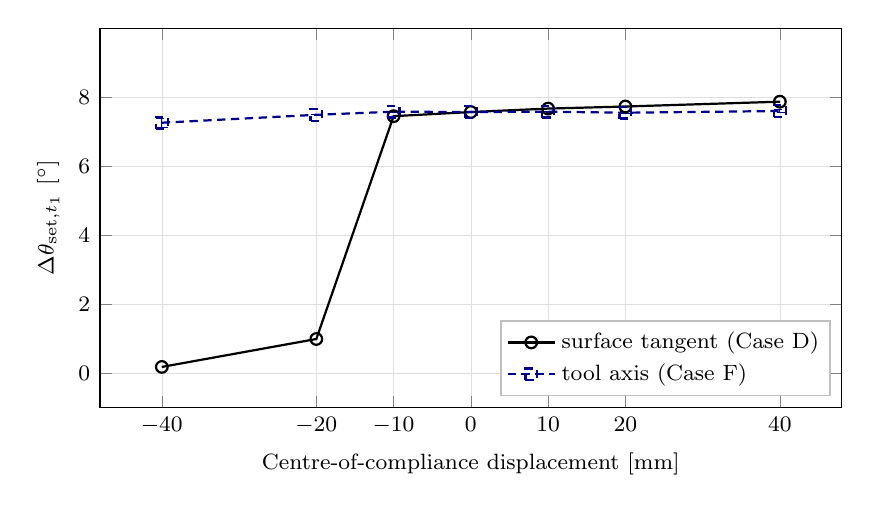
\begin{tikzpicture}
\begin{axis}[
    width=11.0cm, height=6.4cm,
    xmin=-48, xmax=48, ymin=-1, ymax=10,
    xtick={-40,-20,-10,0,10,20,40},
    ytick={0,2,4,6,8},
    grid=major,
    grid style={gray!25, very thin},
    tick label style={font=\footnotesize},
    label style={font=\footnotesize},
    xlabel={Centre-of-compliance displacement [mm]},
    ylabel={\(\Delta\theta_{\mathrm{set},t_1}\) [\(^\circ\)]},
    legend style={font=\footnotesize, draw=gray!50, fill=white,
                  cells={anchor=west}, inner sep=2pt, at={(0.985,0.03)},
                  anchor=south east},
    every axis plot/.append style={thick, mark size=2.1pt},
  ]

\addplot[black, mark=o] coordinates {
  (-40,0.18) (-20,0.99) (-10,7.45) (0,7.57) (10,7.67) (20,7.73) (40,7.87)};
\addlegendentry{surface tangent (Case~D)}

\addplot[blue!55!black, mark=square, densely dashed,
         error bars/.cd, y dir=both, y explicit] coordinates {
  (-40,7.26) +- (0,0.13)
  (-20,7.49) +- (0,0.01)
  (-10,7.58) +- (0,0.01)
  (0,7.57)   +- (0,0.01)
  (10,7.58)  +- (0,0.01)
  (20,7.55)  +- (0,0.03)
  (40,7.60)  +- (0,0.04)};
\addlegendentry{tool axis (Case~F)}

\end{axis}
\end{tikzpicture}
